\subsection{Qualitative Auswertung}
\label{sec:qualitative}

Im Allgemeinen wurde der Block-Editor als übersichtlich beschrieben. Viele Teilnehmer:innen sahen in ihm eine Vereinfachung der Abläufe des Konvertierens und Erstellen von SimplexSzenarios.

Als besonders positiv herausgestellt wurde die Typ-Filterung, mit der die Auswahlmöglichkeiten automatisch auf relevante Einträge reduziert wurden. Vier Teilnehmer:innen beschrieben dies als die beste Funktionalität des Editors. Außerdem wurde mehrfach die Aussage getroffen, dass es einfach sei, Funktionen miteinander zu kombinieren und somit Daten zu transformieren. Im Szenario-Modus wurde die farbige Unterscheidung der Objektklassen als besonders praktisch angesehen.

Es konnte festgestellt werden, dass durch den Block-Editor das bisher benötigte häufige Nachschlagen verhindert wurde. Die Teilnehmer:innen konnten die Aufgaben bewältigen, ohne externe Ressourcen nutzen zu müssen. Ein Verlassen der Anwendung war nicht notwendig, da die benötigten Informationen (verfügbare Ausgangsdaten und Funktionen) innerhalb des Editors verfügbar sind. Drei Teilnehmer:innen wünschten sich jedoch zusätzlich zum Datenschema auch Zugriff auf die Quelldaten selbst zu haben, um sich ein Bild über die enthaltenen Daten zu verschaffen.

Da es im Block-Editor nicht mehr nötig ist, manuell \ac{SQL}-Anweisungen einzutragen, konnten Tippfehler vermieden werden. Einige Teilnehmer:innen stellten dies als positiv hervor. Auch festgestellt werden konnte, dass keine der Abfragen, die als Teil der Testsitzungen generiert wurden, Syntax-Fehler verursachten. Inhaltliche Fehler konnten dadurch nicht vermieden werden, diese traten jedoch nicht häufig auf. Eine Person, die keine Programmier- oder \ac{SQL}-Erfahrung hat, drückte ihre ausdrückliche Freude darüber aus, die getesteten Aufgabenstellungen nun selbst bewältigen zu können.

Die Frage, ob sich die Teilnehmer:innen in der Benutzung der Anwendung effizient fühlten, wurde durchgehend positiv beantwortet. Mehrere Personen gaben an, dass sie die Aufgaben schneller als zuvor absolvieren konnten, und ihre Zufriedenheit anstieg, da weniger manuelle Arbeit nötig war. Als Grund für die Effizienzsteigerung wurde beispielsweise das Auswahlmenü auf der linken Seite genannt, welches häufiges Nachschlagen verhindert. Eine Person drückte als Vorbehalt aus, dass die benötigten Funktionen definiert sein müssen. Sei dies nicht der Fall, könnte es mit der gewählten Herangehensweise zu Problemen kommen, die nur frustrierend zu lösen sind.

\vspace{\baselineskip}

% - positive Sachen
%   - allgemeine beschreibung
%     - übersichtlich
%     - vereinfachung
%   - positiv herausgestellt
%     - Datentypen über Icons
%     - automatisches Filtern x4
%     - funktionen zusammenbauen x2
%     - farbige unterscheidung von Klassen im Szenario-Modus x2
%   - häufiges Nachschlagen wurde verhindert, Aufgaben konnten gelöst werden ohne Quelldaten abzurufen
%     - jedoch wurde sich von 3 Teilnehmer:innen gewünscht, zugriff auf quelldaten zu haben, querverlinkung um eigentlichen inhalt zu sehen
%   - tippfehler
%     - nichts tippen müssen
%     - keine abfragen die fehler verursachten, allerdings paar inhaltliche fehler
%   - no sql
%     - gut dass selbst möglichkeit mapping zu machen
% - effizienz
%   - wahrscienlich ist mensch viel schneller und kann damit mehr machen
%   - wenn es etwas gibt was nicht als funktion definiert ist, wird es scheuslich, in jedem anderen fall schneller
%   - funktionen nicht mehr suchen und wenn das besser wird auf jeden fall produktiver und einfacher, übersicht was es alles gibt super
%   - auf jeden Fall schneller, zufriedenheit wächst weil nicht so viel manuelle arbeit

Im Rahmen der Testsitzungen wurden 20 verschiedene Usability-Probleme identifiziert. Diese wurden entweder im Zuge von \ac{CTA} von den Teilnehmer:innen bemängelt, oder durch Verwirrung, Zögern und fehlerbehaftete Nutzung festgestellt.

\begin{figure}[!ht]
  \colorlet{presentation}{plot1}
  \colorlet{interaction}{plot2}
  \colorlet{content}{plot3}
  \colorlet{technical}{plot4}
  \centering
  \begin{tikzpicture}
    \begin{axis}[
        xbar=0pt,
        xmajorgrids=true,
        xtick={0,...,10},
        xmin=0,
        xmax=6,
        xlabel={Absolute Häufigkeit},
        /pgf/bar shift=0pt,
        legend style={legend cell align=left},
        legend pos=south east,
        axis y line*=none,
        axis x line*=bottom,
        tick label style={font=\footnotesize},
        legend style={font=\footnotesize},
        label style={font=\footnotesize},
        width=.6\textwidth,
        bar width=3.5mm,
        ymin=1,
        ytick={1,...,20},
        ytick style={draw=none},
        yticklabels={
            {\hyperref[p:functionlist]{Übersichtlichkeit Funktionsliste (T)}},
            {\hyperref[p:präfix]{Präfix von Objektklassen (S)}},
            {\hyperref[p:functions]{Details zu Funktionen (R)}},
            {\hyperref[p:queryables]{Benennung Abfragbare Felder (Q)}},
            {\hyperref[p:scroll]{Probleme mit Scrollen (P)}},
            {\hyperref[p:quelle]{Zugriff auf die Quelldaten (O)}},
            {\hyperref[p:filter]{Automatische Typ-Filterung (N)}},
            {\hyperref[p:statisch]{Angabe von statischen Werten (M)}},
            {\hyperref[p:overload]{Auswahl von Überladungen (L)}},
            {\hyperref[p:rechts]{Benennung rechter Bereich (K)}},
            {\hyperref[p:speichern]{Benennung des Speichern-Buttons (J)}},
            {\hyperref[p:parameterübernahme]{Parameterübernahme bei Überladungen (I)}},
            {\hyperref[p:drag]{Drag \& Drop (H)}},
            {\hyperref[p:ersetzen]{Ersetzen von Einträgen (G)}},
            {\hyperref[p:parameter]{Details zu Parametern (F)}},
            {\hyperref[p:meta]{Metadaten von Szenario-Feldern (E)}},
            {\hyperref[p:attribute]{Anzeige von Attributen in Ziel (D)}},
            {\hyperref[p:datentyp]{Datentyp von Szenario-Feldern (C)}},
            {\hyperref[p:icons]{Icons für Datentypen (B)}},
            {\hyperref[p:bedienreihenfolge]{Bedienreihenfolge von Funktionen (A)}},
          },
        area legend,
        y=6mm,
        enlarge y limits={abs=0.625},
        every axis plot/.append style={fill}
      ]
      \addplot[interaction]  coordinates {(0,0)};  \addlegendentry{Interaktion (8)}
      \addplot[presentation] coordinates {(0,0)};  \addlegendentry{Darstellung (7)}
      \addplot[content]      coordinates {(0,0)};  \addlegendentry{Inhalt (4)}
      \addplot[technical]    coordinates {(0,0)};  \addlegendentry{Technisch (1)}

      \addplot[presentation] coordinates {(1,1)};  % Übersichtlichkeit Funktionsliste
      \addplot[content]      coordinates {(2,2)};  % Präfix von Objektklassen
      \addplot[content]      coordinates {(2,3)};  % Details zu Funktionen
      \addplot[presentation] coordinates {(2,4)};  % Benennung Abfragbare Felder
      \addplot[technical]    coordinates {(3,5)};  % Probleme mit Scrollen
      \addplot[content]      coordinates {(3,6)};  % Zugriff auf die Quelldaten
      \addplot[interaction]  coordinates {(3,7)};  % automatische Typ-Filterung
      \addplot[interaction]  coordinates {(3,8)};  % Angabe von statischen Werten
      \addplot[interaction]  coordinates {(3,9)};  % Auswahl von Überladungen
      \addplot[presentation] coordinates {(4,10)}; % Benennung rechter Bereich
      \addplot[presentation] coordinates {(4,11)}; % Benennung des Speichern-Buttons
      \addplot[interaction]  coordinates {(4,12)}; % Parameterübernahme bei Überladungen
      \addplot[interaction]  coordinates {(4,13)}; % Drag \& Drop
      \addplot[interaction]  coordinates {(4,14)}; % Ersetzen von Einträgen
      \addplot[content]      coordinates {(5,15)}; % Details zu Parametern
      \addplot[presentation] coordinates {(5,16)}; % Metadaten von Szenario-Feldern
      \addplot[presentation] coordinates {(5,17)}; % Anzeige von Attributen in Ziel
      \addplot[interaction]  coordinates {(5,18)}; % Datentyp von Szenario-Feldern
      \addplot[presentation] coordinates {(6,19)}; % Icons für Datentypen
      \addplot[interaction]  coordinates {(6,20)}; % Bedienreihenfolge von Funktionen
    \end{axis}
  \end{tikzpicture}
  \caption{Häufigkeit des Auftretens verschiedener Probleme während der Usability-Studie. Gezählt wird die Anzahl der Testsitzungen, in der das jeweilige Problem aufgetaucht ist.}
  \label{fig:problems}
\end{figure}

Abbildung \ref{fig:problems} listet die aufgetretenen Probleme, zusammen mit ihrer Häufigkeit auf. Hierbei wird die Anzahl der Testsitzungen gezählt, in denen das jeweilige Problem aufgetaucht ist. Es wird nicht zwischen der Stärke des Auftretens unterschieden: Von einer Testperson könnte nur ein Verbesserungsvorschlag geäußert worden sein, während eine andere Person durch das Problem eine Aufgabe nicht richtig absolvieren konnte. Außerdem wird der Härtegrad des Problems nicht bewertet. Ein Problem welches häufig auftritt könnte die Nutzer:innen zu einem geringeren Grad beeinträchtigt haben, während weniger häufig auftretende Probleme ein größeres Hindernis darstellen können. Diesbezüglich können sich auch die Meinungen der Teilnehmer:innen unterscheiden.

Die aufgetretenen Probleme können in vier Kategorien unterteilt werden. Diese sind in Abbildung \ref{fig:problems} farblich dargestellt. Außerdem wurde jedem Problem ein Buchstabe zugeordnet (A-T), mit dem die dazugehörige Textstelle identifiziert werden kann. Im Folgenden werden die Probleme, sortiert nach ihrer Kategorie, erläutert.

\subsubsection{Interaktionsprobleme}

Probleme dieser Art sind dadurch charakterisiert, das sie Hürden beim Bedienen der Oberfläche darstellen. Die Nutzer:innen erwarteten beispielsweise eine unterschiedliche Art der Benutzung, oder hatten Schwierigkeiten bestimmte Aktionen auszuführen. Insgesamt wurden acht Interaktionsprobleme festgestellt.

\plabel{p:bedienreihenfolge}
Am Häufigsten wurde die Bedienreihenfolge von Funktionen \textbf{(A)} kritisiert. Der Block-Editor ist so konzipiert, dass zuerst die gewünschte Funktion gewählt, in das Zielfeld eingefügt wird und dann die dazugehörigen Parameter ausgesucht werden. In sechs Testsitzungen wurde dies thematisiert. Zu beachten ist, dass dieses Problem meistens im Zuge der Textverkettung im zweiten Szenario angesprochen wurde (Vgl. Anhang \ref{app:handout}). Ob dies daran liegt, dass es sich beim Großteil der Testsitzungen hierbei um den ersten Kontakt mit Funktionen handelt, oder dass die gleiche Aufgabe oft mithilfe von Operatoren in der Infixnotation gelöst wird, ist unklar. Vier Teilnehmer:innen äußerten sich nicht zur Art und Weise wie Funktionen im Editor eingesetzt werden und kamen ohne Probleme damit zurecht. Sie hatten alle Programmier- oder \ac{SQL}-Kenntnisse. Die restlichen sechs Personen konnten die Aufgabe zwar lösen, wählten zunächst jedoch andere Herangehensweisen oder merkten an, dass sie es gerne auch anders umgesetzt hätten. Drei von ihnen setzten zunächst den ersten Parameter ein, und wollten dann die Funktion darauf anwenden, während eine weitere Person im Nachhinein den Wunsch ausdrückte, dass es zusätzlich zu aktuellen Funktionsweise auch so gehen sollte. Eine von ihnen begründete diese Herangehensweise mit dem von ihr genutzten \ac{GIS}. Für sie war es nicht auf sofort ersichtlich, wie sie zwei Attribute miteinander verknüpfen kann. Zwei weitere Personen wollten im Rahmen der Textverkettung zunächst komplett auf Funktionen verzichten und die benötigten Attribute nacheinander in das Zielfeld klicken. Nachdem dies nicht möglich war, wollte eine von ihnen manuell die Schlüssel aus der Quelltabelle in das Zielfeld schreiben und mithilfe des Textverkettungs-Operator (\texttt{||})\footnote{\url{https://www.postgresql.org/docs/9.1/functions-string.html}} verketten.

\plabel{p:datentyp}
Der Datentyp von Feldern im Szenario-Modus \textbf{(C)} kann über ein Dropdown beim Button zum Hinzufügen von Feldern angepasst werden. Der Standardtyp ist Text. Im dritten Szenario werden Hausnummer abgefragt, welche als Ganzzahl vorliegen, es muss also ein passendes Feld erstellt werden. In fünf Testsitzungen kam es dadurch zu Verwirrungen, da die Teilnehmer:innen ein Textfeld ausgewählt hatten, und somit die Hausnummer nicht einfügen konnten. Das Dropdown zur Typ-Auswahl wurde nicht sofort wahrgenommen, oder mit dieser Funktionalität verbunden. Eine Person bezeichnete das Dropdown zur Typ-Auswahl als "unintuitiv" und schlug vor, die Anpassung des Typs erst nach Hinzufügen des Feldes durchzuführen. Ein weiterer Vorschlag bestand darin, Funktionen zum Konvertieren von Attributen bereitzustellen, oder dies automatisch durchzuführen. In Abbildung \ref{fig:type-dropdown} ist das beschriebene Dropdown zu sehen. Ein:e Teilnehmer:in wünschte sich, die im Rest der Anwendung genutzten Icons auch in diesem Menü wiederzufinden. Während einer Testsitzung wurde der Button für das Hinzufügen von Textfeldern als zu groß empfunden, und vorgeschlagen, alle Datentypen in einem Dropdown unterzubringen, oder den Datentyp des großen Buttons dynamisch anzupassen.

\begin{figure}
  \centering
  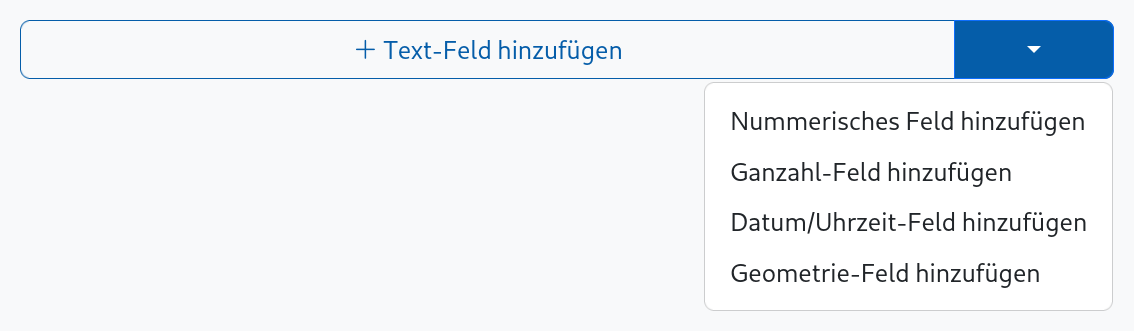
\includegraphics[width=.9\textwidth]{assets/datatype-dropdown.png}
  \caption{Dropdown zum Auswählen des Datentyps von Feldern im Szenario-Modus}
  \label{fig:type-dropdown}
\end{figure}

\plabel{p:ersetzen}
In der Zielstruktur eingetragene Attribute können nicht ersetzt werden \textbf{(G)}. Dies fiel vier Teilnehmer:innen auf. Sie versuchten, durch ein erneutes Anklicken eines bestehenden Eintrages den Inhalt mit einer Auswahl aus dem linken Menü zu überschreiben. Aktuell muss zuerst der Button zum Löschen gedrückt werden, wodurch das Feld wieder frei ist und erneut befüllt werden kann. Eine Person versuchte immer wieder eingetragene Attribute zu ersetzen, obwohl sie bereits festgestellt hatte, das dies nicht möglich ist. Zu beachten ist, dass ausschließlich versucht wurde, Attribute zu ersetzen, keine Funktionen. Dies könnte der Art und Weise geschuldet sein, wie eingetragene Attribute dargestellt sind - sie ähneln einem leeren Feld. In Abbildung \ref{fig:buffet-simple} ist der Unterschied zwischen einem leeren Feld, einer eingetragenen Funktion und einem eingetragenen Attribut zu sehen.

\plabel{p:drag}
Ebenso oft trat es auf, dass Teilnehmer:innen mittels \textit{Drag \& Drop} \textbf{(H)} Elemente von links nach rechts ziehen wollten. In jedem der vier Fälle war es die erste Intuition und wurde ausgetestet. Nach der Realisation, dass \textit{Drag \& Drop} noch nicht implementiert ist, konnte der Großteil zur konzipierten Bedienweise (Auswahl erfolgt von links nach rechts) übergehen. Eine Person tat sich mit der Transition zu dieser Bedienweise schwer.

\plabel{p:parameterübernahme}
Beim Auswählen von Funktionsüberladungen werden die Parameter von einer Überladung nicht in die nächste übernommen \textbf{(I)}. Vier Personen waren davon verwirrt, dass die ersten, bereits ausgefüllten Parameter, leer sind, sobald eine Überladung mit mehr Parametern ausgewählt wird. Zwei von ihnen merkten an, dass die Anzahl der Parameter auch nach dem Ausfüllen anpassbar sein sollte, wobei eine von ihnen darauf einging dass es schwierig sein könnte, dies konsistent umzusetzen. Ein:e Teilnehmer:in erkannte, dass die zuvor eingetragenen Parameter in der Überladung mit weniger Parametern bestehen bleiben, und entfernte diese manuell, aus Angst dass dies Fehler verursachen könnte.

\plabel{p:overload}
Von den Personen, die keine Probleme mit den Parametern von Überladungen hatten, benutzten drei die Überladungs-Funktionalität gar nicht. Sie erkannten die Möglichkeit nicht, eine andere Überladung auszuwählen \textbf{(L)}. In Abbildung \ref{fig:concat-overload} und \ref{fig:concat-nested} ist die Funktion \texttt{concat} zu sehen, bei der es zu den genannten Problemen kam. Die drei Personen, die keine Überladungen benutzten, wählten die in Abbildung \ref{fig:concat-nested} abgebildete Herangehensweise, die zur Folge hat, dass $n-1$ mal die Funktion ausgewählt werden muss, wobei $n$ die Anzahl der Einzelbestandteile ist. Zwei der drei Personen nahmen dies so hin, während die dritte es als "nervig" und "umständlich" bezeichnete. Im Nachhinein wies sie auch darauf hin, dass sie die Pfeile zum Umschalten zwischen Überladungen als ungeeignet erachtet. An dieser Stelle hätte sie eher ein Plus und Minus erwartet, oder vielleicht sogar ein Plus am Ende der Parameterliste platziert. In einer anderen Testsitzung wurde der in Abbildung \ref{fig:concat-overload} zu sehende Tooltip ("nächste Überladung verwenden") kritisiert, da die meisten Menschen nicht wissen, was Überladungen sind.

\begin{figure}[!ht]
  \minipage[t]{.49\textwidth}
  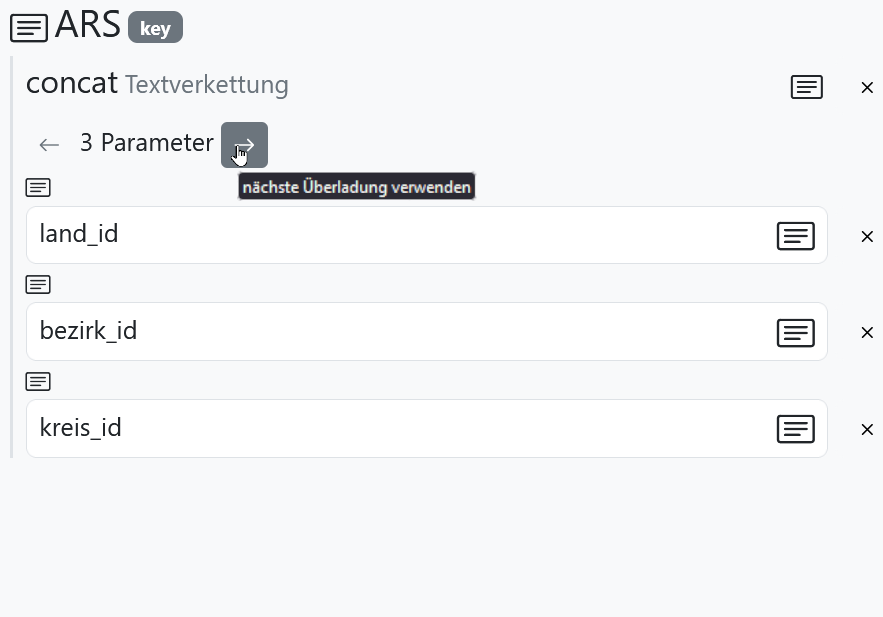
\includegraphics[width=\linewidth]{assets/concat-overload.png}
  \caption{Überladung der Funktion \texttt{concat} (vier Parameter). Der angezeigte Tooltip lautet "nächste Überladung verwenden".}
  \label{fig:concat-overload}
  \endminipage
  \hfill
  \minipage[t]{.49\textwidth}
  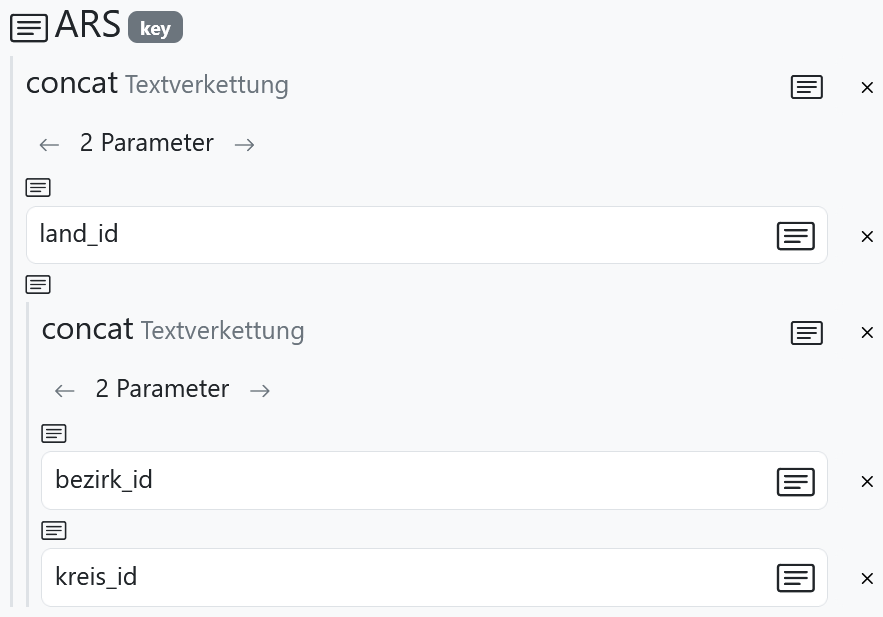
\includegraphics[width=\linewidth]{assets/concat-nested.png}
  \caption{Eine geschachtelte Version der Funktion \texttt{concat}.}
  \label{fig:concat-nested}
  \endminipage
\end{figure}

\plabel{p:statisch}
Die Angabe von statischen Werten \textbf{(M)} führte in drei Testsitzungen zu zwei unterschiedlichen Problemen. Statische Werte können anstelle von Attributen oder Funktionen in Eingabefeldern eingegeben werden. Dabei kann der Wert ohne besonderen Syntax eingegeben werden, da es sich im Block-Editor um an den Datentyp angepasste Eingabefelder handelt. Eine Person war sah eine einfache Eingabe nicht als Option an und war sich nicht im Klaren dass dies möglich ist. Zwei weitere Teilnehmer:innen setzten ihre Texteingabe zunächst in Hochkommas, konnten diesen Fehler dann jedoch am Ende relativ schnell beheben. Die beiden zuletzt genannten Personen haben Programmier- und \ac{SQL}-Kenntnisse und nannten diese als Ursprung ihrer Handlung.

\plabel{p:filter}
Der Block-Editor filter automatisch relevante Auswahlmöglichkeiten basierend auf ihrem Datentyp \textbf{(N)}. In drei Testsitzungen wurde diese Funktionalität missverstanden. Im extremsten Fall konnte die Testperson nichts mit den Datentypen anfangen, und war somit auch nicht in der Lage das Konzept des automatischen Typ-Filters zu verstehen. In einer anderen Testsitzung wurde zwar realisiert, dass beim Anklicken von Elementen links in der Zielstruktur Felder deaktiviert werden, dieser Effekt wurde allerdings dem falschen Grund zugeschrieben. Die Person war der Meinung, dass der Grund hierfür eine bereits getätigte Auswahl ist. In diesem Fall führte dies dazu, dass die durch die Filterung verursachten Änderungen in der UI nicht transparent wirkten. Auffällig war, dass alle drei Teilnehmer:innen von links nach rechts arbeiteten, das heißt, es fiel ihnen schwerer den vollen Effekt der Filterfunktion zu verstehen. Eine dieser Personen äußerte sogar den Wunsch, die Liste der Funktionen zu filtern, erkannte aber nicht, wie dies funktioniert. Wenn die Oberfläche von rechts nach links benutzt wurde, trat dieses Problem nicht auf, es gab aber auch Teilnehmer:innen, die von von links nach rechts arbeiteten, und denen die Funktionsweise klar wurde. Eine:r von ihnen ging daraufhin sogar dazu über, zuerst das Feld rechts auszuwählen, und dann das einzufügende Element links auszusuchen.

\subsubsection{Darstellungsprobleme}

Auch die Darstellung von Informationen innerhalb des Block-Editors führte zu Problemen. Es wurden acht Darstellungsprobleme identifiziert, welche von unklaren Bezeichnungen bis hin zu Icons reichen.

\plabel{p:icons}
Abbildung \ref{fig:icons} zeigt die vom Block-Editor verwendeten Icons für Datentypen \textbf{(B)}. Diese werden wie in Abbildung \ref{fig:attribute-source} und \ref{fig:attribute-target} verwendet, um über den Datentyp von Attributen, Funktionen und Feldern zu informieren. Im Rahmen von fünf Testsitzungen wurden die Icons missverstanden oder führten zu Verwirrungen. Da sich die Icons für Ganz- und Gleitkommazahlen nicht voneinander unterscheiden, kam es zu Verwechslungen. Eine Person wählte beispielsweise im dritten Szenario ein Gleitkommazahl-Feld aus (im Dropdown als "numerisch" bezeichnet, siehe Abbildung \ref{fig:type-dropdown}), um eine Hausnummer einzusetzen, obwohl es sich bei der Hausnummer um eine Ganzzahl handelt.  Drei Teilnehmer:innen sahen das Icon für Booleans als zwei interaktive Schalter an, und versuchten, sie zu bedienen. Eine Person empfand das Icon für den Datentyp Text als Button, über den mehr Informationen über ein Attribut oder eine Funktion abgerufen werden könnten. Eine weitere Person empfand die Icons als guten Ort, um einen Ausschnitt aus der Quelltabelle abzurufen.

\begin{figure}
  \centering
  \begin{tikzpicture}
    \tikzset{icon/.style={outer xsep=4.5em, outer ysep=1em, minimum height=3em}}
    \tikzset{label/.style={font=\footnotesize}}
    \node [icon] (text)  at (0, 0)       {\includesvg[width=2em]{assets/bi-card-text.svg}};
    \node [icon] (int)   at (text.east)  {\includesvg[width=2em]{assets/bi-123.svg}};
    \node [icon] (float) at (int.east)   {\includesvg[width=2em]{assets/bi-123.svg}};
    \node [icon] (bool)  at (float.east) {\includesvg[width=2em]{assets/bi-toggles.svg}};
    \node [icon] (dt)    at (bool.east)  {\includesvg[width=2em]{assets/bi-calendar-week.svg}};
    \node [icon] (geom)  at (dt.east)    {\includesvg[width=2em]{assets/bi-pin-map.svg}};
    \node [label] at (text.south)  {Text};
    \node [label] at (int.south)   {Ganzzahl};
    \node [label] at (float.south) {Gleitkommazahl};
    \node [label] at (bool.south)  {Boolean};
    \node [label] at (dt.south)    {Datum/Zeit};
    \node [label] at (geom.south)  {Geometrie};
  \end{tikzpicture}
  \caption{Die im Block-Editor verwendeten Icons für Datentypen \parencitealias{bootstrapIcons}.}
  \label{fig:icons}
\end{figure}

\plabel{p:attribute}
Die Anzeige von Attributen in der Zielstruktur weicht von der im Auswahlmenü ab \textbf{(D)}. Im Auswahlmenü wird sowohl der Name, als auch der Schlüssel von Attributen angezeigt, während im rechten Bereich nur noch der Schlüssel angezeigt wird. Dies fiel fünf Teilnehmer:innen auf, zumeist im dritten Szenario, wahrscheinlich weil sich dort die Inhalte mehr unterscheiden. Abbildung \ref{fig:attribute-source} und \ref{fig:attribute-target} stellen dies beispielhaft dar. "strassenname" ist der Name des Attributs der Objektklasse, während "description" der Schlüssel ist. Sobald das Attribut im Ziel erscheint, wird nur noch der Schlüssel angezeigt. Besonders im Fall der Standardfelder \footnote{\texttt{key, ndx, typ, dsc, cmt, beg, fin}, Vgl. \ref{sec:theory-s4d-reality}}, kann dieser stark vom Name abweichen. Fünf Personen waren davon verwirrt.

\begin{figure}[!ht]
  \minipage[t]{.38\textwidth}
  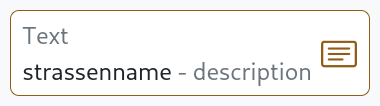
\includegraphics[width=\linewidth]{assets/attribute-source.png}
  \caption{Ein Attribut im Auswahlmenü.}
  \label{fig:attribute-source}
  \endminipage
  \hfill
  \minipage[t]{.60\textwidth}
  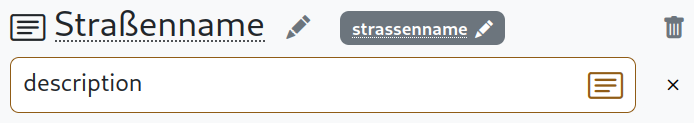
\includegraphics[width=\linewidth]{assets/attribute-target.png}
  \caption{Ein Attribut in der Zielstruktur - es wird nur der Schlüssel dargestellt.}
  \label{fig:attribute-target}
  \endminipage
\end{figure}

\plabel{p:meta}
Im Szenario-Modus besteht die Möglichkeit, grundlegende Metadaten der Felder zu bearbeiten \textbf{(E)}. Wie in Abbildung \ref{fig:attribute-target} zu sehen, können Titel (\texttt{nam}, "Straßenname") und Schlüssel (\texttt{key}, "strassenname") bearbeitet werden. Dies soll sowohl über die Stift-Symbole als auch durch die gepunktete Linie unter den Werten signalisiert. Die Möglichkeit der Bearbeitung wurde nicht immer wahrgenommen. In zwei Fällen wurden die Standardwerte so belassen wie sie sind. In fünf Testsitzungen kam es jedoch zu verschiedenen Komplikationen während der Bearbeitung der Metadaten. Der Unterschied zwischen den zwei Werten war den Teilnehmer:innen nicht bekannt und oft wurde deshalb nur der Titel angepasst. In einem Fall trat jedoch das Gegenteil ein - als Grund wurde genannt dass der Schlüssel durch den dunklen Hintergrund mehr hervorstach. Eine Person verwechselte den Schlüssel (\texttt{key}) mit der Beschreibung (\texttt{dsc}), welche allerdings nicht über die Anwendung editierbar ist. Zwei mal wurde vorgeschlagen, den Schlüssel über eine \texttt{slugify}-Funktion anhand des Titels zu generieren, um Mehrfacheingaben zu verhindern. Auch kritisiert wurde, dass nicht ersichtlich ist, dass es sich beim Schlüssel um ein Pflichtfeld handelt und dass der Inhalt beim Beginn der Bearbeitung nicht automatisch komplett ausgewählt ist.

\plabel{p:speichern}
Als Abschluss von Szenarios sollten die Teilnehmer:innen den "Speichern"-Button \textbf{(J)} betätigen, und so zur in Abbildung \ref{fig:scenario-result} dargestellten Tabellenansicht gelangen. In der Aufgabenstellung wurde vermieden, die in der Anwendung verwendete Sprache zu nutzen. Es wurde nur der Hinweis gegeben, dass die erstellten Objekte überprüft werden sollen. Nicht in allen Testsitzungen konnte erfolgreich die Assoziation zwischen der Beendigung der Aufgabe, dem Überprüfen des Resultats und dem "Speichern"-Button geknüpft werden. Insgesamt vier Personen waren mit der Benennung des Buttons unzufrieden, wobei zwei von ihnen spezifizierten, dass sie durch das Klicken auf "Speichern" nicht erwarteten, die Eingaben überprüfen zu können oder eine Vorschau zu sehen. Ein:e Teilnehmer:in würde "Ausführen" als eine angemessenere Benennung empfinden. Zu beobachten war, dass Personen, die bereits mehr Erfahrung mit der Benutzung von Simplex4Data hatten, die Benennung des Buttons nicht kritisierten. Der Button zum Speichern von Formularen ist in Simplex4Data standardmäßig oben rechts zu finden.

\plabel{p:rechts}
Wie bereits während der Einfindungsphase bemerkt, kam es bezüglich der Identifikation des rechten Bereiches \textbf{(K)} zu Problemen. Während der Szenarios identifizierten drei Personen zuerst fälschlicherweise die Zielstruktur als Quelltabelle, und brauchten somit länger, um die allgemeine Funktionsweise des Block-Editors zu verinnerlichen. Ein:e Teilnehmer:in äußerte als Grund für die Verwirrung, dass sie nicht wusste, dass Standardfelder umbenannt werden können. Eine weitere Person erkannte zwar auf Anhieb, dass es sich bei den Feldern im rechten Bereich um die Zielstruktur handelt, wünschte sich jedoch trotzdem eine Überschrift zur Orientierung.

\plabel{p:queryables}
Bei zwei der drei eben beschriebenen Testsitzungen wurde die Benennung der abfragbaren Felder in der Seitenleiste bemängelt \textbf{(Q)}. Das passierte während des ersten Szenarios, in dem die abfragbaren Felder die Felder der Quelltabelle darstellen. Deshalb wurde vorgeschlagen, diesen Abschnitt klarer zu benennen, zum Beispiel als Quell- oder Importtabelle. Eine Behebung dieses Problems könnte auch zu einer einfacheren Einfindung führen.

\plabel{p:functionlist}
Eine Person empfand die Liste der Funktionen im linken Menü als zu unübersichtlich \textbf{(T)}. Dies erschwerte ihr das Finden von relevanten Funktionen, und weckte das Gefühl, dass die Funktionen fachspezifischer wären. Ein während der Testsitzung geäußerter Lösungsvorschlag lautete, die Funktionen in Themenbereiche zu unterteilen, um primitivere, beziehungsweise häufiger genutzte, Funktion hervorzustellen.

\subsubsection{Inhaltliche Probleme}
In einigen Testsitzungen wurde festgestellt, dass ein verbesserter inhaltlicher Kontext zum erfolgreichen Abschließen von Aufgaben hilfreich sein kann. Im Gegensatz zur vorherigen Kategorie werden Inhalte hier nicht unbedingt verwirrend dargestellt, sondern existieren gar nicht in der Oberfläche.

\plabel{p:parameter}
\begin{figure}[!ht]
  \centering
  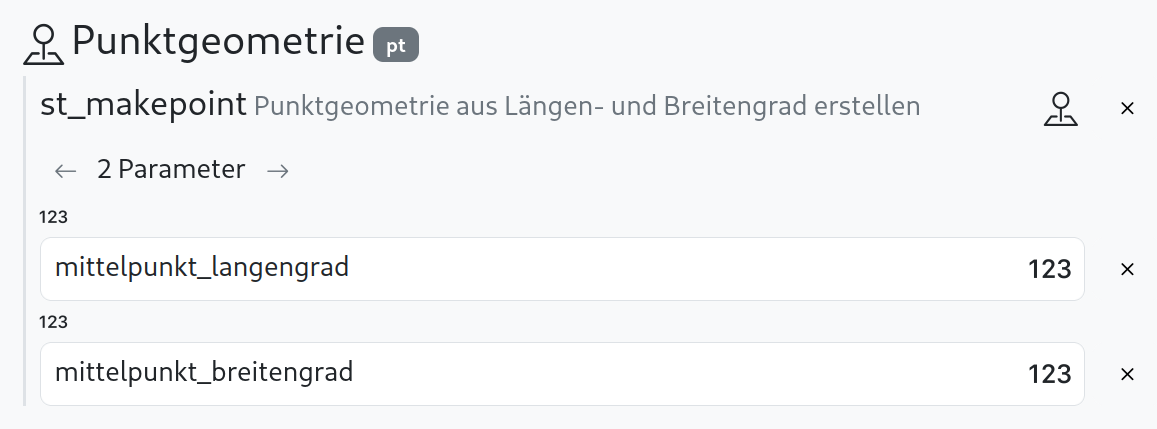
\includegraphics[width=.9\textwidth]{assets/st-makepoint.png}
  \caption{Die Funktion \texttt{ST\_MakePoint} mit korrekt ausgefüllten Parametern.}
  \label{fig:parameters}
\end{figure}
Im zweiten Szenario musste die Funktion \texttt{ST\_MakePoint} benutzt werden, um aus Längen- und Breitengraden eine Punktgeometrie zu bilden. Hierbei fehlte es an Details zu den benötigten Parametern \textbf{(F)}. Bis auf eine Teilnehmer:in war allen klar, dass die Reihenfolge der Parameter von Relevanz ist, fünf konnten jedoch nicht sofort feststellen, in welcher Reihenfolge die Parameter ausgefüllt werden müssen. Abbildung \ref{fig:parameters} zeigt die besagte Funktion, ausgefüllt in der korrekten Reihenfolge. Die Beschreibung nennt die Parameter in der richtigen Reihenfolge. Eine Person sah dies als Hinweis an, drückte jedoch aus, dass die Parameter trotzdem beschriftet werden sollten. Zwei weitere Personen äußerte eine ähnliche Meinung, während in einer anderen Testsitzung der Hinweis innerhalb der Beschreibung bevorzugt wurde. Ein:e Teilnehmer:in schlug ein Pop-Up für eine detailliertere Beschreibung der Parameter vor. Falls die Parameter für \texttt{ST\_MakePoint} falsch gesetzt wurden, fiel dieser Fehler spätestens beim Betrachten der Ergebnisse in der Tabellenansicht auf, und konnte durch ein Austauschen behoben werden. Die Teilnehmer:innen zeigten Unsicherheit in Bezug auf die Reihenfolge der Parameter und erwarteten dies somit als Fehlerquelle.

\plabel{p:quelle}
Im Zuge von drei Testsitzungen wurde der Wunsch geäußert, eine Vorschau der Quelldaten zu sehen \textbf{(O)}. Dies würde den Teilnehmer:innen helfen, die Ausgangsdaten zu verstehen und zu wissen dass die ausgewählten Datentransformationen richtig sind. Die genannte Hürde trat beispielsweise während des zweiten Szenarios auf, als der amtliche Regionalschlüssel (\acs{ARS}) gebildet wurde. Es stand die Frage im Raum, ob führende Nullen aufgefüllt werden müssen, oder ob diese bereits existieren. Ein Person wünschte sich, Werte der einzelnen Attribute abrufen zu können, während eine weitere eine tabellarische Darstellung über alle Attribute bevorzugen würde. Zu guter Letzt fasste ein:e Teilnehmer:in die Möglichkeiten zusammen: Es könnte eine Schnittmenge aller Daten gezeigt werden, oder nur verschiedene Werte von den einzelnen Attributen. Die zuletzt genannte Person schlug auch das Icon für den Datentyp als Ort vor, um solche Informationen abzurufen.

\plabel{p:functions}
Zwei Personen wünschten sich eine detailliertere Beschreibung der Funktionen \textbf{(R)}. Als Grund wurde genannt, dass manche Funktionsnamen nicht aussagereich genug sein könnten, insbesondere für Personen mit weniger Fach- oder Programmiererfahrung. Genannte Lösungsvorschläge beinhalten Tooltips und Pop-Ups, zum Beispiel über einen Button mit dem Buchstabe \textit{i} als Symbol.

\plabel{p:präfix}
\begin{figure}[!ht]
  \centering
  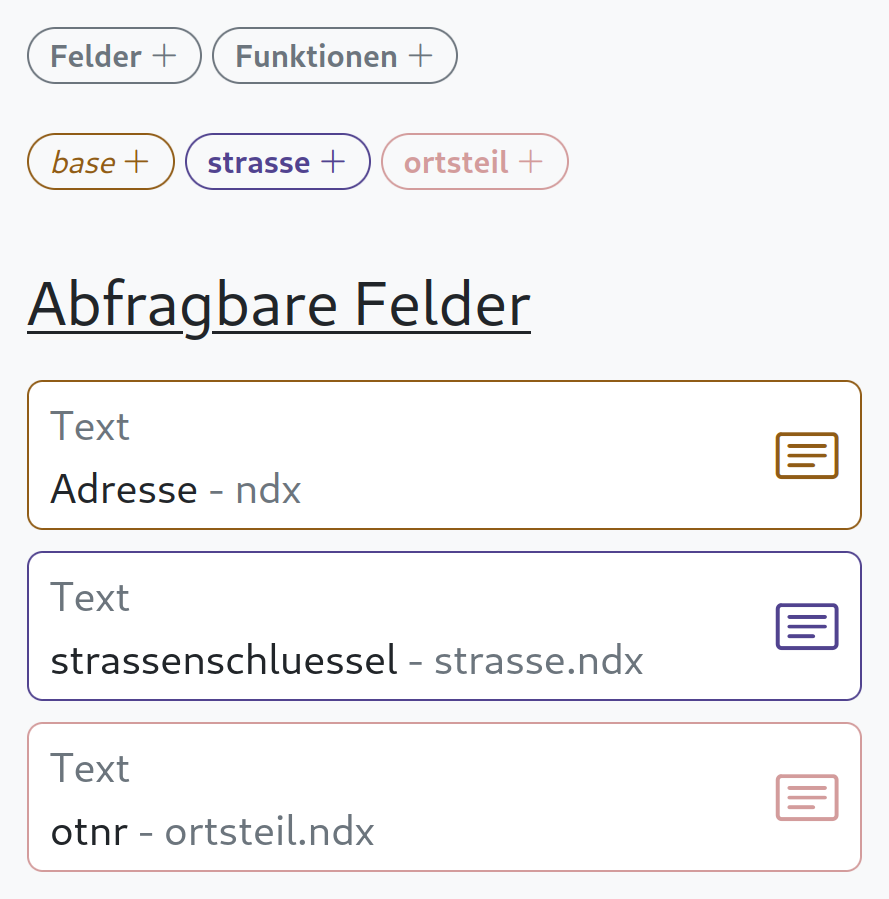
\includegraphics[width=.5\textwidth]{assets/scenario-prefixes.png}
  \caption{Das Standardfeld \texttt{ndx} für drei Objektklassen im dritten Szenario. Die Objektklasse "Adresse" ist Ausgangspunkt des SimplexSzenarios und verfügt über keinen Präfix. Im Filtermenü (oben) wird diese Klasse als \textit{base} bezeichnet.}
  \label{fig:scenario-prefixes}
\end{figure}
Im Szenario-Modus besitzen die Attribute von verbundenen Objektklassen einen Präfix \textbf{(S)}. Nur die zentrale Objektklasse folgt diesem Schema nicht - die Attribute werden ohne Präfix ausgeliefert. Dies führte bei zwei Personen zur Verwirrung, da im dritten Szenario die Klasse "Adresse" keinen Präfix hatte, und somit nicht so leicht identifizierbar wie die anderen Klassen war. Außerdem konnte eine der beiden Teilnehmer:innen die Bezeichnung "base" im Filtermenü für den rechten Bereich nicht der zentralen Objektklasse zuordnen. Abbildung \ref{fig:scenario-prefixes} zeigt für die Objektklassen im dritten Szenario, wie das gleiche Standardfeld in verschiedenen Klassen dargestellt wird. Im oberen Bereich ist auch das Filtermenü sichtbar.

\subsubsection{Technische Probleme}
Im Laufe der Usability-Studie traten kaum technische Probleme auf. Falls die allgemeine Funktionsweise des Block-Editors beeinträchtigt wurde, konnte dies vor Anfang der Szenarios gelöst werden, beispielsweise durch das Ausschalten eines aktiven \acs{VPN}s.

\plabel{p:scroll}
Während einer Usability-Studie fiel auf, dass das Scroll-Verhalten unter Chrome nicht optimal ist \textbf{(P)}. Es war zwar der komplette Inhalt zu sehen, sobald jedoch im rechten Bereich ans untere Ende und darüber hinaus gescrollt wurde, bewegte sich die gesamte Anwendung nach oben. Zwei weitere Teilnehmer:innen, die nicht Chrome benutzten, äußerten den Wunsch die Zielstruktur ein bisschen weiter nach oben scrollen zu können, damit am unteren Ende mehr Platz ist. Eine von diesen Personen nannte als Grund dafür, dass auf ihrem Laptop der untere Teil des Browser-Fensters verdeckt wurde.
